\chapter{分析根因} % Introduction chapter suppressed from the table of contents

先用日本俱乐部里由7位年轻女服务员组成的QC圈在84年做改善的故事介绍根因分析的主要元素。

\framebox{%
\begin{minipage}[t]{0.97\columnwidth}\raggedright
\textbf{根因分析(Causal Analysis \& Resolution CAR)的主要步骤:}

\begin{enumerate}
\tightlist
\item
  选择要分析的结果, 利用二八原则识别引起大部分问题的最主要因素
\item
  分析背后的主要根因
\item
  对应改进措施(改进建议)
\item
  评价改进效果
\item
  总结成根因分析报告(A3报告)\\
\end{enumerate}

可参考附件A:``绅士俱乐部过程改进''了解团队如何按以上步骤做过程改进的实例。
\strut
\end{minipage}}

\hypertarget{ux6839ux56e0ux5206ux6790ux7684ux8befux89e3}{%
\section{根因分析的误解}\label{ux6839ux56e0ux5206ux6790ux7684ux8befux89e3}}

请千万不要误以为只要使用了根因分析的方法（例如：二八原则）就能做好，很多团队在开始时对其理解可能只是一知半解，需要不断纠正和改进。\\
某公司过程改进组（共4人）对过去一年的项目进行了根因分析，旨在改进交付质量，减少交付验收时的缺陷数。\\
%\href{文件:Epg-car3.1-1.png}{600px}\\

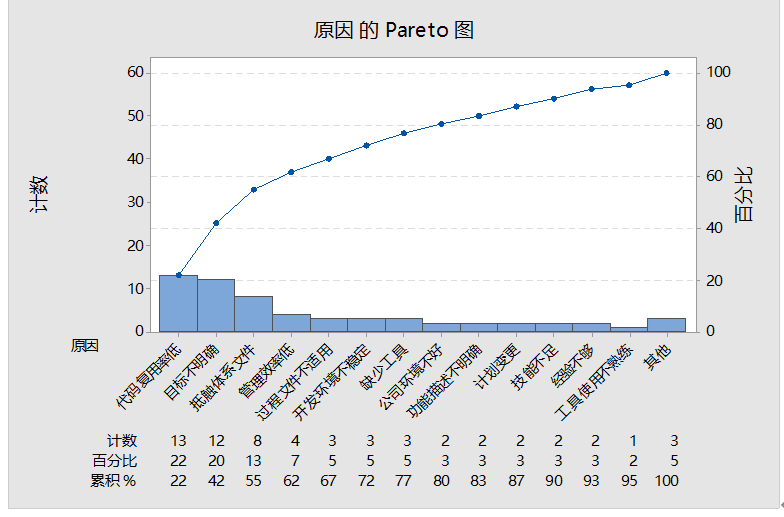
\includegraphics[width=10cm]{Epg-car31-1.png}
图11-5

我：请问这帕累托图的依据？\\
组长：针对客户缺陷密度较高的现状，我们做了敏感度分析。发现需求引入的缺陷数跟它相关性最高，接下来我们使用鱼骨图分析，请4个人一起头脑风暴，共识别出十几项主要原因种类。然后按每人3票的原则，各自单独投票得出排序。最后根据二八原则，我们识别出前3项主要原因，接着，我们根据这3项原因又进一步发现，这些原因是导致需求缺陷的原因，包括流程图画不好等。\\
香港启德国际机场1996年航班延误统计：\\
%\href{文件:CRairportDelayScreenshot_2023-06-02_191306.jpg}{600px}

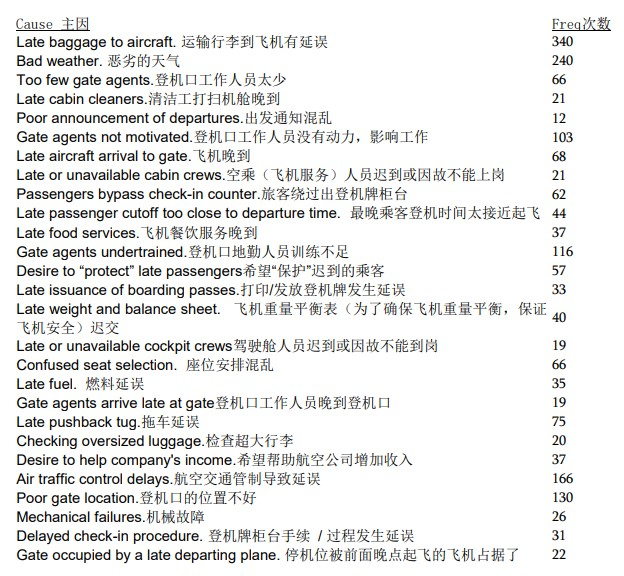
\includegraphics[width=10cm]{CRairportDelayScreenshot_2023-06-02_191306.jpg}

图11-6

然后我解释：\\
我们不应直接把几十条原因按他们对问题的影响度从最高排到最低做帕累托图，而应先对原因进行分类。
以机场延误为例，我们需要区分哪些是不可抗力的天然原因（如天气原因），哪些是与闸口管理相关的问题，哪些是与机场打印登机牌相关的问题。
例如，如果识别出与闸口管理相关的问题最多，后续就可以针对这些问题进一步分析根因。
分析才能有针对性。（详见附件）\\
你们的分类和帕累托图依据的``数据''都不过是用数字来表达你们头脑风暴的主观判断，所以这种帕累托图其实与直接用头脑风暴做出的结论没什么差异。
你们只是用投票数据使结果看起来``量化''了，但其实并没有客观数据支撑。\\
你们的分类存在问题。
例如只有``功能描述不明确''，难道``非功能需求描述不明确''（如性能、安全性等）就不需要考虑吗?\\
你们现在的分类有不少是重复的，同样一个问题有可能归属于2、3个分类。\\
你们的度量操作定义也存在问题。例如，如何根据历史项目的数据判断哪些原因归属于``功能描述不明确''？\\
建议你们应该首先识别出与想要解决的问题相关的度量项，针对这些度量项收集数据，然后再做分析。
收集客观数据才是根因分析的第一步。

\hypertarget{ux6309ux56e2ux961fux6c34ux5e73ux56e0ux624dux65bdux6559}{%
\section{按团队水平因才施教}\label{ux6309ux56e2ux961fux6c34ux5e73ux56e0ux624dux65bdux6559}}

``发现我讲过的方法总是需要重复解释和提醒，是不是我教的方法有问题？''
某老师交流时问道。\\
``这很正常，绝不要怀疑方法本身，我也经常遇到类似的情况。实际上，这是一切学习的必经过程：起初只是根据学到的技巧初步应用到项目中，而要实现持久应用，不仅需要团队持续实验才能真正理解，还离不开`奴、徒、工、匠、师、家、圣'这个不断学习的过程。''

下面是针对根因分析，与他分享各团队水平不同，辅导方式不同的故事。

\begin{description}
\tightlist
\item[]
= = = = = = = =
\end{description}

\hypertarget{ux9ec4ux5e26ux6c34ux5e73}{%
\subsection{黄带水平}\label{ux9ec4ux5e26ux6c34ux5e73}}

某家专门做企业管理产品的软件开发的Y公司：\\
总经理听完如能做好迭代回顾和根因分析，不仅可以大大减少后期返工的工作量、提升产品质量，还能够提高整体开发效率，很感兴趣，并说会要求工程部按这思路做改进。\\
8个月后再次见面时，总经理说：``虽然我们现在已经要求团队多做回顾和根因分析，但每次迭代的系统测试缺陷数量还是降不下来。比如某产品线，每次迭代的缺陷数量大约在50个左右，也曾降到过30个左右，但不久之后又回到了之前的水平。能否跟我们团队谈谈，了解一下情况？''

\begin{description}
\tightlist
\item[]
= = =
\end{description}

我：第二条根因是什么？\\
团队答：编码人员把某个参数搞混了。

\begin{description}
\tightlist
\item[]
改进措施：提醒开发人员要注意，避免同类问题再发生
\end{description}

第一条是测试人员不清楚需求，没有设计出充分的测试用例，导致未能在测试阶段预先暴露问题

\begin{description}
\tightlist
\item[]
改进措施：加强人员的培训，更了解业务需求
\end{description}

我：测试本身是不会产出缺陷的，为什么你们识别测试是根本原因的源头呢？

\begin{description}
\tightlist
\item[]
= = =
\end{description}

以上是与团队交流的节录。\\
从他们提供的缺陷数据、缺陷分析和系统测试报告等材料，发现他们并没有真正找到根本原因，只是对缺陷进行了分类，并针对缺陷暴露出的问题，提出了修正措施。\\

\framebox{%
\begin{minipage}[t]{0.97\columnwidth}\raggedright
团队自认为在复盘时已经做了根因分析，但虽然有参加过根因分析培训，但还是误以为对应发现的问题都做了处理便分析了根因。
如果他们听完夜总会例子后，再小组分析机场延误数据，就能帮助他们先了解根因分析的基础。
\strut
\end{minipage}}

\begin{description}
\tightlist
\item[]
= = = = = =
\end{description}

X公司主要为全国不同的医院开发医疗行业的软件产品。六年前，公司规模还不到五百人；四年前，公司办公地点扩大了一倍，占地3000平方米，总人数也增加到接近900人。尽管公司骨干比较稳定，但新人的流动性很大。公司制定了很多量化指标，如需求一次性通过率、开发速度、测试缺陷密度等，并不断监控，但并未取得明显改善。\\
技术总监问：``请教一个一直困扰我的问题------如何激励团队，让他们更有积极性？''\\
``现在你们员工的收入底薪和奖金的比例大概是多少？''\\
总监：``大概七成底薪，其他的就按每人每年的表现分发。''\\
``主要依赖主管的打分吗？我完全可以理解为什么是这个结果了。因为在这种安排下，员工的收入既不会太差，但也不会特别高，所以他们自然缺乏动力去改进自己的工作表现。''\\
总监解释：``也不完全依赖主管的主观判断。我们制定了很多与绩效相关的度量指标，以根据这些指标客观地计算员工的奖金多少。''\\
``理解了，你觉得这样便能客观吗?
一旦把度量与绩效/奖金挂钩，就会导致收集不到真实的数据。因为只要数据与收入有关联，高层需要什么数据，下面都会提供，这完全失去了度量的本意。收集度量数据本来希望像镜子一样，让团队可以看到现在的真正水平。团队成员相互合作非常重要，所以日本公司通常不会发奖金给某个个人，而是发给团队。团队的奖金应该与团队为公司提供的价值（换算成金额）挂钩，这样才客观透明。大家可以预估到如果团队有了提升，能为公司赚多少钱，自己收入大概会增加多少。除了金钱上面的奖励，也不要忽略非金钱的赞赏，例如，定期让项目团队分享改进成功的故事，也可以帮助团队持续改善。你们每个开发团队里面都有明确的分工：需求、开发、测试等都有相关的度量指标。但岗位之间缺乏交流，导致团队的整体质量和效率没有显著提升，例如团队的缺陷密度和返工率一直没有明显下降。''\\
接下来，我讲述了60年代美国费城的Weisbord先生针对印刷公司订单管理部使用XY理论改革团队的故事：如何从每一步骤都要按小主管(supervisor)安排的传统管理模式（X型管理），变为由4-5人自我管理的独立团队（Y型管理），最终把每天处理订单量提升50\%的成功改革故事。\\
总监说：``听完这个故事，确实感觉我们团队的管理模式类似于X型管理。虽然我们团队每两周进行一次迭代，但没有真正做到团队合作。测试人员只负责测试，开发人员只写程序，然后交给测试人员去测试。因此，从这个角度看，或许每个过程的指标，如测试和开发都很好，但团队的整体能力没有任何提升。''\\
``从这次观察来看，每个迭代中，系统测试的缺陷数保持在40-60个左右，六个月前是这个水平，现在依然如此，现在还是这个水平，没有任何进步。为什么？因为大家缺乏团队协作和互补的团队精神，导致没有改进的动力。各岗位只顾管好自己，确保指标达标，不被扣绩效就行。''因为我也对团队缺乏具体改进感到失望，所以不管总监是否高兴，我直言不讳地指出问题。\\

\framebox{%
\begin{minipage}[t]{0.97\columnwidth}\raggedright
如果没有可信的数据，大家了解了根因分析的基础也不会促进改善，应先解决怎样能收集到真实数据这问题。
\strut
\end{minipage}}

\hypertarget{ux7effux5e26ux6c34ux5e73}{%
\subsection{绿带水平}\label{ux7effux5e26ux6c34ux5e73}}

虽然X公司团队已经接受了根因分析的培训，并且在每次迭代回顾中都在使用，但依然遇到挑战。以下是项目团队分享会里的交流：``第一条根本原因写的是`开发人员不理解需求，没有按照规格要求，导致后续测试不通过。'请举例说明。''\\
``我们这个项目是系统升级，针对医生在手术前的很多准备工作，不仅包括麻醉师，还包括护士、设备等都需要准备就绪。而且大小医院要求不同，大医院分工很细，小医院可能由一个岗位负责多个任务。所以，要避免此类缺陷，首先要画出所有可能的处理流程图，明确有哪些不同的配置项和参数，并与熟悉流程的产品经理（甚至医生）确认。''\\
``这些内容是否都应该归入根因分析的范围呢？还记得我们之前讲过的 KJ
分析方法吗？（详见附件）所有团队成员需要用便利贴写下所有相关的因素和问题，并在大白纸上画出它们之间的关系，这才算是完整的根因分析。你现在写的``根本原因''只是浮在水面上现象。\\
再看对应的纠正措施：记得我们一直强调，改进计划也要像项目管理一样，用WBS将任务分解成不超过五天的可执行部分，并明确任务负责人。每个任务都必须有具体的产出物。如果只简单写成``一个月后由开发组长负责完成''，但由于缺乏实际行动，最终一个月后很难取得理想的效果。''


\resizebox{\linewidth}{!}{

\renewcommand{\arraystretch}{1.5}

\begin{tabular}{|c|c|c|c|}
\hline
\:& 根本原因 & 纠正措施 & 行动计划\\
\hline
1) & 开发人员不理解需求，没有按照规格要求，导致后面测试不通过 &
开发与需求改善开发前的沟通，加强相关业务培训 & 7.17 (一个月后
)，张XX（开发组长）\\
\hline
2) & 接口测试出错，没有使用正确接口，不清楚接口参数（2349，2321） &
代码评审时检查接口相关检查 & 7.17 (一个月后
)，张XX（开发组长）\\
\hline
3) &
开发没有充分自己测试好，很多非一般，但可能出现的情况，报错或显示效果不好。开发要加强自测（2419，2421，2412，2433）
& 对开发人员加强相关测试培训 & 7.17 (一个月后 )， 李XX（项目经理） +
王X（系统测试）\\
\hline
\end{tabular}

}



``我们分析根本原因都应有要数据支撑，不应单依赖个人主观判断。这里第三项根因只是写了四个缺陷号，是什么意思？''\\
``因为我们没有时间把几十条缺陷都列出来分析，我们只能抽几条把缺陷号记下来。''\\
``你们总共有多少时间做迭代回顾？''\\
``一小时左右。''\\
``明白了。确实时间不够，所以管理层必须给你们充分的时间，不然的话，无法做好根本原因分析。''\\
``第二条写`没有使用正确接口'是什么问题？''\\
``这系统有很多外部接口与医院现有系统对接，有些缺陷是因为开发一测试用的接口版本不同，导致测试时不通过。''\\
``记得我们一直强调，开发、测试与客户的生产环境必须一致，因此这是一个关于环境的问题，接口只是环境的一部分。那么，为什么会出现版本错误？是否不应仅靠人工记录最新版本的对应关系？你们现在代码开发版本在Git管理；但相关文档，包括配置，在SVN管理。依赖人工记录这些之间的相互对应，很容易出错，这才是根因。''

虽然团队经过培训，已经理解了根因分析的原理，但还是不太了解如何用于实际工作中。这类的定期分享会，加上咨询老师的辅导会有帮助。

\hypertarget{ux5206ux6790ux5168ux8fc7ux7a0b}{%
\subsubsection{分析全过程}\label{ux5206ux6790ux5168ux8fc7ux7a0b}}

为北京某企业进行差距分析时，发现大量缺陷在系统测试阶段才被发现，因此建议加强迭代回顾中的根因分析。\\
质量经理：你说我们上次做了回顾还没有找到真正根因，但不知道如何改善。\\
我：数据是根因分析的基础，若要做好分析，首先要有充分和足够数据。\\
例如，团队只依据系统测试缺陷数据进行分析，由于没有缺陷对应的返工工作量的数据，只能从缺陷类型的数量来分析，这使得难以识别出影响最大的缺陷类别。\\
此外，没有考虑从需求设计开始进行评审、编码人员的自测，也没有关注各阶段的缺陷排除率，结果大家只能从系统测试缺陷的症状进行分析，结论是编码人员疏忽或能力不足，而不会考虑这些缺陷是否可以在早期预防和避免。\\
因此，在每次迭代回顾时，我们必须给团队足够的时间来收集数据，绘制全流程图以识别失效点，这对分析也有帮助。\\
流程图不仅能帮助分析过程，还能帮助找出根因。绘制流程图后，就可以利用
FMEA 方法针对每个失效点找出根因和相应的纠正措施。

\framebox{%
\begin{minipage}[t]{0.97\columnwidth}\raggedright
某公司专门为电信供应商开发客服管理软件系统。由于客户对软件质量要求较高，因此每次发布后都会对发现的问题进行分析。某些与软件开发相关的问题不易查明根因，例如某次发布后，发现报表中的数字对不上。然而，这些错误并不是开始使用时就出现的，刚开始使用时一切正常，但时间长了错误就显现出来了。\\
团队花费了大量时间分析整个过程，最终发现问题的根源在于某些内部接口未能充分考虑到传输的数据是否正常。部分数据虽然有误，但未被拒收，这导致系统在初期表现正常，但随着有问题的数据逐渐累积，最终引发了报表错误。\\
在讨论如何避免类似问题时，团队提出了以下改进措施：

%\href{文件:微信截图_20230928135611.png}{500px}

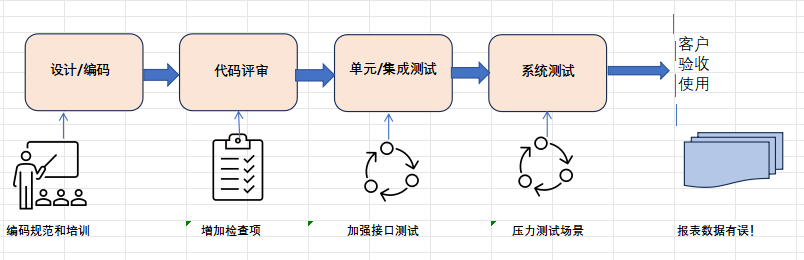
\includegraphics[width=10cm]{微信截图_20230928135611.png}

按照系统产品集成的流程思路，可以参考FMEA的思路识别哪些环节可以预防问题的发生。为了减少类似问题的出现，可以在集成测试和系统测试阶段增加类似的场景，并加大压力测试的力度，以提前暴露潜在问题。在集成测试中，全面测试所有接口传输的数据也能有效防止问题发生。如果我们做好了前期的设计和代码评审（问题的根源往往与设计有关），也能预防类似情况的出现。例如，通过完善评审检查单的检查项，以后应该能够避免同类问题再次发生。
\strut
\end{minipage}}

从这个实例可以看出，首先绘制总体流程或路线图，并识别每个环节的潜在风险，有助于更好地挖掘问题的根本原因。

\hypertarget{ux5982ux4f55ux5206ux6790ux4e0eux5bf9ux5e94ux5404ux7c7bux7531ux4e8eux4ebaux5458ux5f15ux8d77ux7684ux7f3aux9677}{%
\subsection{如何分析与对应各类由于人员引起的缺陷}\label{ux5982ux4f55ux5206ux6790ux4e0eux5bf9ux5e94ux5404ux7c7bux7531ux4e8eux4ebaux5458ux5f15ux8d77ux7684ux7f3aux9677}}

\begin{itemize}
\tightlist
\item
  可大致分为4类跟人相关的缺陷和对应措施
\end{itemize}

\resizebox{\linewidth}{!}{

\renewcommand{\arraystretch}{1.5}

\begin{tabular}{|c|c|c|c|}
\hline
类 & 分析后发现缺陷模式 & 可能的根因 & 解决办法\\
\hline
1 & 某些缺陷，发生模式是随机的，不容易看出哪类缺陷经常发生。 &
错误是由于疏忽造成的。 & 完善过程，防止人为错误。\\
\hline
2 & 某些缺陷，有些人员经常犯错，但另一些人员总是``很好''。 &
错误是由于缺乏技巧造成(能力、知识、技能等)。例如某些窍门只有部分人知道。
& 挖掘和推广窍门，避免出现小众才知道的秘密。\\
\hline
3 & 有些人员总是在各种各样的缺陷上容易犯错。 &
潜在的原因：故意不遵守标准。天生不能完成这类任务。缺乏培训。 &
激励措施。换人。提供培训。\\
\hline
4 & 某些缺陷，所有工人都容易犯错。 & 缺陷是应该由管理层控制。 &
语言标准化；提供翻译，词汇表。达到自我控制标准。\\
\hline
\end{tabular}

}



表11-7

实例1：

表11-8统计了6位技术人员，按29种缺陷统计：

%\href{文件:Juran_t5.8.jpg}{文件:Juran t5.8.jpg}


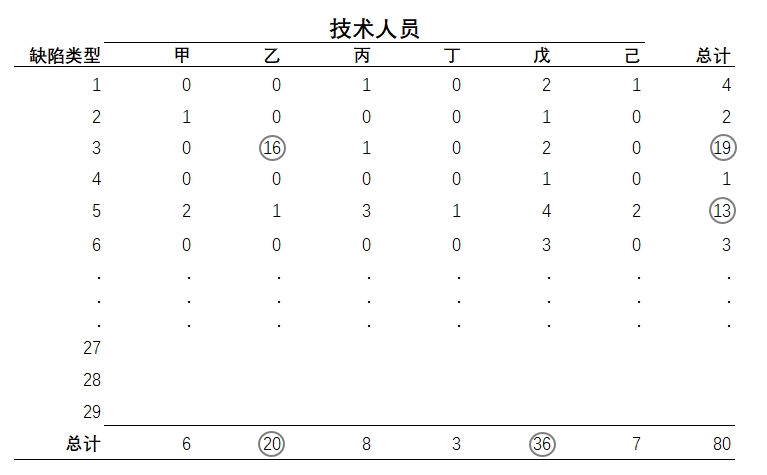
\includegraphics[width=10cm]{Juran_t58.jpg}

表11-8

分析：\\
*虽然第3类缺陷出现共19次（最多），但大部分是源自员工乙，但他除了犯类型3缺陷外，他其他方面的缺陷数很少。很可能是他误解了里面某些关键过程（表11-8的类型2）

\begin{itemize}
\tightlist
\item
  第5类缺陷属于上表的第4类，所有员工都有犯错
\item
  员工戊的缺陷数最多，占了缺陷总数接近一半，是表11-8中类型2的例子
\end{itemize}

实例2：来福枪故事

\begin{itemize}
\tightlist
\item
  是上面类型3的标准例子
\end{itemize}

软件开发绝大部分靠人来完成，也可以从``人''的维度分析，例如：

\begin{itemize}
\tightlist
\item
  下面是22位来福枪组装工人从2月到7月的缺陷数统计，他们每人负责完整安装一支抢：\\
\end{itemize}

\begin{description}
\item[]
\begin{description}
\tightlist
\item[]
（缺陷：试验后无法打开，取出空弹壳。导致必须从组件重新安装。）
\end{description}
\end{description}

%\href{文件:Juran_t5.10.1.jpg}{文件:Juran t5.10.1.jpg}

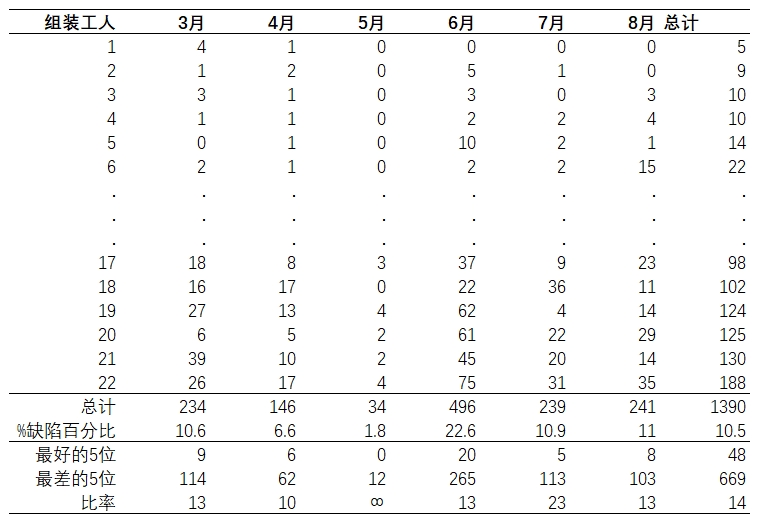
\includegraphics[width=10cm]{Juran_t5101.jpg}

表11-3

\begin{description}
\tightlist
\item[]
发现每月的缺陷率差异很大（从1.8
到22.6）；但发现6个月里最差5位与最佳5位缺陷数的比例差不多。所以不是个别人员能力的差异，而应是有原因。\\

观察最佳和最差工人的工作方法发现质量好的工人都会用金属打磨器对负责的逐渐打磨。最差的工人都没有这样做。\\
\end{description}

\hypertarget{ux603bux7ed3}{%
\subsection{总结}\label{ux603bux7ed3}}

利用机场延误数据做小组练习，了解根因分析的基础后，可以用FMEA分析全过程找根因，也可以从人员的缺陷分析找出与人员相关的根因。

是否表示如果能把握好各种根因分析技巧，便可以避免问题或灾难发生?

\framebox{%
\begin{minipage}[t]{0.97\columnwidth}\raggedright
\textbf{太空穿梭机（航天飞机）灾难} （Space Shuttle
disasters)
1986:
挑战者号（Challenger）航天飞机升空后，于发射后的第73秒爆炸，机上7名宇航员全部罹难(
相关视频可以在网上搜到)。直接原因是用来密封火箭液态氢气燃料缸的O型橡胶环在摄氏零度低温不能及时膨胀。但这事故并非偶然。升空前，供应商已经警告过低温会影响橡胶的性能；以前的实验也发生过橡胶环有些部分半径只能达到预期的2/3。但管理层为了按计划预期升空都漠视这些安全隐患预警。\\2003：哥伦比亚号
(Columbia)
航天飞机在返回地球时，因为左翼的隔热保护胶在16天前升空时被固体火箭助推器外层脱落的乳胶击破损坏，导致航天飞机返航时进入大气层的第1000秒钟，在35,000米高空因过热解体，7名宇航员全部罹难。\\
Ride在2003哥伦比亚号灾难事故调查回顾说
：我很诧异这两次事故的原因非常相似（她也是挑战者号事故调查组员），86年引起挑战者灾难的陋习又再出现
:
为了赶上计划升空日期，而忽略了之前性能报告的发现，没有注意前线技术工程人员提出的安全隐患，也缺乏安全保障措施。其实从哥伦比亚号在1981年首次升空开始，每次都有出现升空时燃料缸外的保护乳胶掉落的事故，但管理层一直都没有关注，工程师因为赶进度，每次升空前，都没有时间预先处理好。\\ 虽然调查报告有找出事故的根因，但过了几年后，管理层只关注项目的成本与进度，忽略了质量与安全，没有再注意调研报告指出隐患，事故还是重复发生。

\strut
\end{minipage}}

NASA资源丰富，内部不缺经验丰富的工程师，工程师都了解各种根因分析技巧，但管理层为了赶进度，忽略了多次质量预警，最终因为发生了这两次致命事故，航天飞机计划最终被叫停。所以如果领导只关注进度，忽视质量，缺少风险意识，团队都懂得应如何做好根因分析，也不会有作用。\\

\hypertarget{ux9644ux4ef6}{%
\section{附件}\label{ux9644ux4ef6}}

\hypertarget{ux673aux573aux5ef6ux8befux6570ux636eux5206ux6790}{%
\subsection{机场延误数据分析}\label{ux673aux573aux5ef6ux8befux6570ux636eux5206ux6790}}

行李延误数量最多（340），但如果按以下分组：

\begin{itemize}
\tightlist
\item
  闸口
\item
  行李运输
\item
  飞机（包括机组人员，燃料等）
\end{itemize}

发现闸口相关的总数反而比行李运输高。
%\href{文件:!11airportAnalysis_Screenshot_2024-11-09_160632.jpg}{500px}

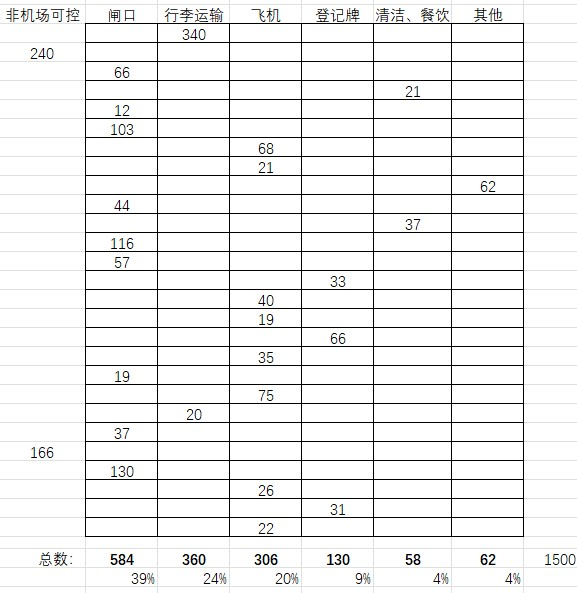
\includegraphics[width=10cm]{!11airportAnalysis_Screenshot_2024-11-09_160632.jpg}

前3类的总数： 83\%(=39\% + 24\% + 20\%)

\hypertarget{fmea-ux5b9eux4f8b}{%
\subsection{FMEA 实例}\label{fmea-ux5b9eux4f8b}}

\begin{description}
\tightlist
\item[]
(FMEA: Failure Mode Effects Analysis)\\
\end{description}

大家可能都经历过因为没有管理好时间而导致迟到的情况。以坐飞机为例，从离开酒店到登上飞机的过程中，很可能因为一些风险导致最后没搭上飞机。\\
当你出发时，可能选择不同的交通方式，如出租车或机场大巴。如果你不能在起飞前45分钟到达机场办理登机牌，你就无法登机。但即使你拿到了登机牌，也有可能最后没能搭上飞机，因为机组严格执行起飞前15分钟关舱门的规定，所以你还需要在起飞前15分钟到达登机口。\\

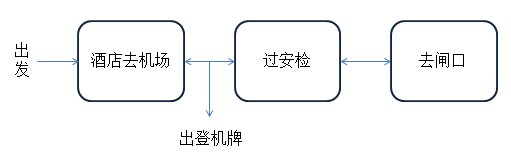
\includegraphics[width=10cm]{风险与机会1.png}

图11-7 登机过程

要赶上飞机其实是个过程，中间有很多环节会导致最后失败，所以我们可以通过FMEA过程分析来看如何减少失败的概率。

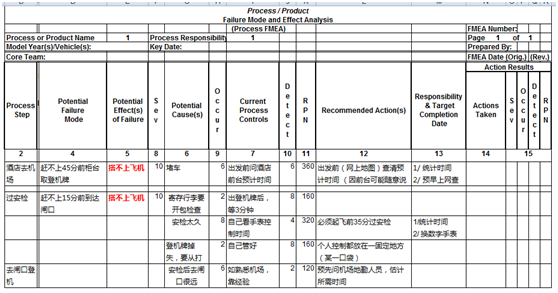
\includegraphics[width=10cm]{风险与机会2_FMEA.png}

表11-4 FMEA 例子

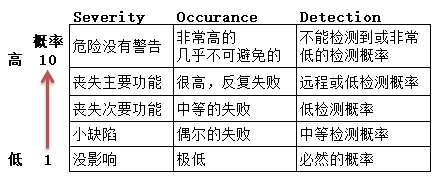
\includegraphics[width=10cm]{226页替换图片.jpg}

表11-5 打分参考

以第一个失效为例：如果发生就会坐不上飞机，所以严重性最高，评分为10。发生的概率比较高，评分为6。是否容易预防、预警？由于不熟悉当地情况，加上主要依靠酒店前台提供信息，而有时他们也不清楚，所以评分为6。RPN
=10×6×6=360。\\
从以上登机的例子可以看出，FMEA是以整个过程进行风险管理的。比如在出发前，就要查询一下各个交通工具要花费的时间，例如，在出发前，需要查询各个交通工具所需的时间。在南京，从酒店坐地铁需要转车，要花费一个小时以上，如果时间紧张就会来不及，那么宁可多花钱打车，以控制风险。\\
即使拿到了登机牌，还需要经过安检并到达登机口。有时机场很大，到达登机口也要花很长时间，因此需要提前问好路径并计算好时间，避免误点。\\
如果从安检到登机口需要超过10分钟，那么就需要在起飞前35分钟通过安检，才能来得及。这些都可以通过FMEA的形式把整个坐飞机的过程识别出来，找出各个阶段可能出现的问题，从而知道如何控制。\\
以这个坐飞机的风险为例，我自己就多次没赶上飞机。原因很多，但总结一下，都是因为习惯没有改过来。我应依据以往差点赶不上的经验，回顾一下，确保每一个过程都控制住，就不会后面再次出问题
，这个和企业做风险管理概念一样。\\
有度量才有管理。人和公司一样，很多事情看似是自己主动去想的，其实很多都是潜意识的习惯。如果没有设定一些量化的控制手段，就不会提高这方面的风险意识，还是会错过飞机。因此，我通过回顾以往几次搭飞机的情况，把每次到达机场的时间和到达登机口的时间记录下来（详见下面图4）。\\
上面是机场柜台关闭（45分钟）前到达时间，下面是关闸口前到达时间（分钟）（X代表赶不上飞机）:

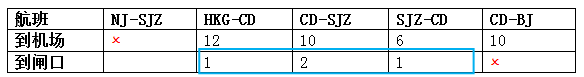
\includegraphics[width=10cm]{风险与机会41.png}

表11-6

最近一次赶不上飞机是因为未能在关闸门前到达，而之前也有两次类似情况------我刚到闸口，就到时间马上关闸了。\\
如果我把经验教训记下来，下次做好时间管理，就会避免后面的延误：有了数据，我们便可以更有效在回顾时做好根因分析
(CAR)。\\
以这登记延误风险为例，可以使用FMEA分析每个失效点，例如过安检（因没有预留足够时间）和从安检到闸口所需时间太长等的发生概率都很高（前者为8，后者为6）。\\
为了避免问题再发生，就要定一些具体的计划，最终希望把误点减到零。\\
在登机这个环节，可以利用以下有效方法/工具来帮助改善：\\
*每次出发去机场前都查询各种交通方式的时间与风险（概率），预留足够时间，降低失效发生的概率\\
*拿到登机牌后，计划好在起飞前35分钟通过安检\\
在多次错过飞机后，我发现传统手表没有正负5分钟的准确性，而使用电子手表可以精确到正负1分钟，这有助于更好地把控时间。

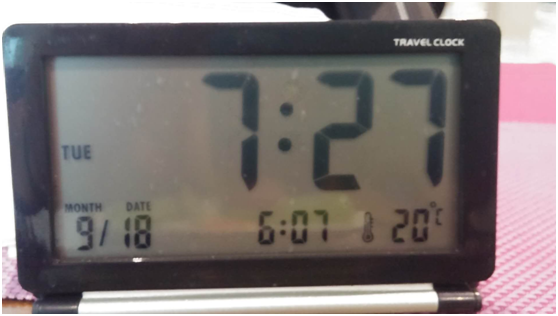
\includegraphics[width=10cm]{风险与机会5_闹钟.png}

图11-8 平常用于培训/评估计时的电子钟

经过这次误机，我就买了个电子手表，取代传统针式手表，希望对日后不迟到有帮助。\\
\textbf{效果}：这件事发生在2019年9月，之后我按这些计划行动，再没有出现赶不上飞机的情况。我每次都提醒自己必须在起飞前60
\textasciitilde{} 90分钟到机场，30 \textasciitilde{}
45分钟前到闸口。分析的目的是提高个人风险意识，避免问题发生。

